\chapter{Sistemi di telecomunicazione}\label{sec:sistemi-di-telecomunicazione}\index{sistema di telecomunicazione}

\section{Obiettivi del corso}

Applicando la teoria dei segnali si vogliono acquisire la capacità di progettare sistemi di telecomunicazione per la trasmissione dell'informazione da una sorgente ad un ricevitore su un canale trasmissivo garantendo un sufficiente livello di accuratezza in presenza di fenomeni di disturbo.

Un sistema di telecomunicazione tra una \keyword[sistema di telecomunicazione!sorgente]{sorgente} dell'informazione e un \keyword[sistema di telecomunicazione!destinatario]{destinatario} è modellato per componenti: un \keyword{trasmettitore}, un \keyword[sistema di telecomunicazione!canale di trasmissione]{canale di trasmissione}, un \keyword[sistema di telecomunicazione!ricevitore]{ricevitore}. Il messaggio contenente l'informazione generata alla sorgente $m(t)$ viene trasmesso sul canale di trasmissione e ricevuto come $\tilde{m}(t)$ al destinatario. Ogni passaggio può alterare il contenuto del messaggio che viene elaborato, filtrato, affetto da disturbi, non linearità, attenuazione e distorsione. Per ricostruire il messaggio originale è necessario che tali modifiche siano reversibili.

Per sistemi analogici l'informazione è generata, elaborata e trasmessa come onda elettromagnetica. Nei sistemi digitali l'informazione è rappresentata da stringhe di bit alla sorgente che il trasmettitore trasforma in onde elettromagnetiche per la trasmissione.

\begin{figure}[!ht]
\centering
\resizebox{\textwidth}{!}{
\begin{tikzpicture}[node distance=3.5cm,minimum width=2.5cm,text width=2.5cm,align=center, >=latex'];
\node [block](t1) {Elaborazione del segnale};
\node [block,right of=t1](t2) {Modulatore}edge[<-](t1);
\node [block,right of=t2,node distance=5cm,minimum height=1em](c) {Mezzo Tx};
\node [fitted,fit=(t1) (t2),label=above left:Trasmettitore] {};
\node [fitted,fit=(c),label=above:Canale]{};
\node [above of=c,node distance=1.5cm,pin=above:Rumore](n) {$n(t)$}edge[->](c);
\node [block,right of=c,node distance=5cm](r1) {Demodulatore};
\node [block,right of=r1](r2) {Elaborazione del segnale}edge[<-](r1);
\node [fitted,fit=(r1) (r2),label=above left:Ricevitore] {};
\node [left of=t1,node distance=3cm,minimum width=1.5cm,text width=.5cm,pin=below:Informazione in ingresso](m1) {$m(t)$}edge[->](t1);
\node [right of=r2,node distance=3cm,minimum width=1cm,text width=.5cm,pin=below:Dati per l'utente](m2) {$\hat{m}(t)$} edge[<-](r2);
\draw [->] (t2)--node[above]{$s(t)$}(c);
\draw [->] (c)--node[above]{$r(t)$}(r1);
\end{tikzpicture}
}
\caption{Schema di principio di un sistema di TLC}\label{fig:schema_sistema_telecomunicazioni}
\end{figure}

L'informazione prodotta dalla sorgente in forma analogica o digitale viene elaborata dal trasmettitore per ottenere un segnale adattato al mezzo di trasmissione: segnali con spettri in \keyword[spettro!in banda base]{banda base} concentrati attorno alla frequenza nulla possono essere trasmessi direttamente su canali passa basso, che lasciano passare non attenuate le frequenze nella banda base. Se il canale risulta già utilizzato a tali frequenze o se per caratteristiche del canale tali frequenze sono troppo attenuate o distorte è possibile modulare ovvero traslare lo spettro del segnale nella \keyword[spettro!in banda passante]{banda passante} del canale trasmissivo. \footnote{Se la potenza a frequenza zero è nulla è assente il segnale in componente continua}

In base alle frequenze utilizzabili nel canale e alla tipologia di trasmissione per mezzo di conduttori o via radio i mezzi trasmissivi si distinguono per tecnologia di canale ad onde elettromagnetiche convogliate o ad onde irradiate e per la risposta in frequenza nei canali passa basso o passa banda.

Ogni componente del sistema di telecomunicazione, a causa di vari fenomeni fisici, è affetto da \keyword[sistema di telecomunicazione!rumore]{rumore} elettronico che altera il segnale in modo indesiderato. Tale segnale di disturbo aleatorio è sovrapposto al segnale contenente l'informazione, ne altera il contributo in potenza a varie frequenze, e risulta indistinto dal segnale utile e causa un \keyword[sistema di telecomunicazione!tasso di errore di trasmissione]{tasso di errore di trasmissione} caratteristico del sistema di telecomunicazione, o \ac{BER} nei sistemi di trasmissione numerica. 

In ogni punto del sistema di telecomunicazione sarà possibile misurare il rapporto segnale rumore (\ac{SNR}). La progettazione di un sistema di telecomunicazione ha lo scopo di dimensionare ogni componente del sistema al fine di minimizzare la potenza necessaria a trasmettere l'informazione stabilendo un rapporto segnale rumore (\ac{SNR}) tale che sia soddisfatto il tasso di errore per sistemi analogici o il \ac{BER} per sistemi numerici digitali.

\begin{table}[!ht]\centering
	\begin{tabular}{c|p{0.3\textwidth}|p{0.3\textwidth}}
		\hline \rule[-2ex]{0pt}{5.5ex}  & Onde Convogliate & Onde Irradiate \\ 
		\hline \rule[-2ex]{0pt}{5.5ex} \keyword{LP} & \parbox[c]{5cm}{Doppino telefonico\\ Cavo coassiale} &  \\ 
		\hline \rule[-2ex]{0pt}{5.5ex} \keyword{BP} & Fibra Ottica & Mezzo Radio \\ 
		\hline 
	\end{tabular} 
	\caption{Tipologie di mezzi trasmissivi}\label{tab:mezzi-trasmissivi}
\end{table}

\section{Rumore}
Nel corso di \textsc{Fondamenti delle Telecomunicazioni} si adotterà l'ipotesi semplificativa di avere sempre un disturbo o rumore descritto da un processo aleatorio \emph{gaussiano bianco}. Tale modello dato dalla sovrapposizione di un gran numero di eventi elementari è valido per frequenze $f\ll\SI{10}{\giga\hertz}$. Si considereranno due tipologie di rumore.

\begin{definizione}
Il \textbf{rumore termico} gaussiano bianco è originato dall'agitazione termica degli elettroni. Per frequenze sufficientemente piccole si hanno i seguenti spettri di potenza:
\begin{equation}\begin{split}
N_W(f)=k_B T \,[\si{\watt\per\hertz}] &\quad \text{spettro potenza monolatero}\footnotemark\\
N_V(f)=4 k_B T R \,[\si{\volt\squared\per\hertz}] &\quad \text{spettro potenza a vuoto}
\end{split}\end{equation}
\footnotetext{ costante di Boltzmann $k_B=\SI{1.3806488e-23}{\joule\per\kelvin}$}
\end{definizione}
\begin{definizione}
\textbf{Rumore granulare} generato dal movimento di cariche elettriche attraverso una barriera di potenziale (es. giunzione $np$):
\begin{equation}\begin{split} N_I(f)= 2 q I [\si{\ampere\squared\per\hertz}]\quad\text{spettro potenza monolatero} \end{split}\end{equation}
\end{definizione}

\section{Rumore in catene di amplificazione}
Si ipotizza una catena di amplificatori nel ricevitore, ognuno dei quali modifica il segnale amplificando di un fattore l'ampiezza del segnale.

Si assume che i dispositivi siano a carichi adattati, ovvero abbiano la medesima impedenza alla porta (l'equivalente di Thevenin o di Norton del circuito). Essendo ogni resistore affetto da rumore termico si ha all'uscita la somma del rumore presente in ingresso amplificato da ogni stadio della catena di amplificatori. Il rumore introdotto da un amplificatore o catena di amplificatori può essere riportato in modo equivalente all'ingresso.

Possiamo usare due modelli equivalenti di rumore in catena di amplificazione.

\begin{figure}[t]
	\centering
	\subfloat[Modello additivo]{
	\begin{circuitikz}[scale=.6,american currents]
		\draw[dashed] (3,4)--(3,-1)node[below]{$k T_g$} (7,4)--(7,-1)node[below]{$k T_s$};
		\draw (2,0)--(0,0)	to[I=${T_g}$] (0,3) to[short,-o] (3,3) --(5,3) (6,3) to[short,-o] (7,3)--(8,3) to[R, l=${R_L}$] (8,0)--(7,0) (5,1.5) node[block,minimum height=3cm]{\parbox{1.5cm}{\centering$A$\\ $T_a$}}
		(2,3) to[R, l=${R}$] (2,0) to[short,-o] (3,0)--(5,0) (6,0) to[short,-o] (7,0);
	\end{circuitikz}\label{fig:modelli_eq_rumore_additivo}
	}\quad\subfloat[Modello fattore di rumore]{\begin{circuitikz}[scale=.6,american currents]
		\draw[dashed] (3,4)--(3,-1)node[below]{$k T_g$} (7,4)--(7,-1)node[below]{$k T_s$};
		\draw (2,0)--(0,0)	to[I=${T_0}$] (0,3) to[short,-o] (3,3) --(5,3) (6,3) to[short,-o] (7,3)--(8,3) to[R, l=${R_L}$] (8,0)--(7,0) (5,1.5) node[block,minimum height=3cm]{\parbox{1.5cm}{\centering$A$\\ $F$}}
		(2,3) to[R, l=${R}$] (2,0) to[short,-o] (3,0)--(5,0) (6,0) to[short,-o] (7,0);
	\end{circuitikz}
	\label{fig:modelli_eq_rumore_moltiplicativo}}
	\caption{Modelli equivalenti di rumore in catena di amplificazione}
\end{figure}

\subsubsection{Modello equivalente di rumore additivo in catena di amplificazione}

\begin{itemize}
	\item Amplificatore con guadagno di potenza $A$
	\item Temperatura equivalente di rumore dell'amplificatore $T_a$ \footnote{ $T_a$ è funzione della frequenza ma per ipotesi semplificativa si considera costante}
	\item Temperatura equivalente di rumore del sistema $T_s=T_g+T_a$ 
	\item Densità spettrale di rumore in uscita all'amplificatore 
	\begin{equation} h_n=k(T_g+T_a)=k T_s \,[\si{\watt\per\hertz}] \end{equation}
\end{itemize}

\subsubsection{Modello equivalente di rumore moltiplicativo in catena di amplificazione}
\begin{itemize}
	\item Fattore $F$ di rumore dell'amplificatore
	\item $F$ è definito ad una data temperatura $T_0$ dell'impedenza (es. $T_0=\SI{293}{\kelvin}$)
	\item Densità spettrale di rumore in uscita
	\begin{equation} h_n=F k T_0 \end{equation}
\end{itemize}

Se $T_g=T_0 \implies F k T_0 = k(T_0+T_a) \implies T_a=(F-1) T_0 \quad F=1+\frac{T_a}{T_0}$

\subsubsection{Catene di amplificazione}
\begin{figure}[!ht]
	\centering
	\begin{tikzpicture}[start chain=going right,node distance=8mm,>=latex',every node/.style={on chain},every join/.style={->},	block/.style={draw,align=center,minimum width=3em}]
	\node[join]{$k T_g$};
	\foreach\i in{1,2,3} {
		\node[sum,join]{$+$};
		\begin{scope}[start branch=above,every join/.style={<-,thick,shorten <=1pt}]
			\node[on chain=going above,join]{$k T_{A_\i}$};
		\end{scope}
		\node[block,join]{$A_\i$};
	}
	\coordinate[join](end);
	\end{tikzpicture}
	\caption{Catena di 3 amplificatori di potenza con modello additivo di temp. equiv. di rumore}
	\label{fig:catena_amplificazione}
\end{figure}

La temperatura equivalente di rumore della catena di amplificazione di potenza in fig.\ref{fig:catena_amplificazione} si ottiene riportando all'ingresso del I stadio tutti i contributi.

\begin{equation}\label{eq:temp_eq_rumore}
T_A=T_{A_1}+\frac{T_{A_2}}{A_1}+\frac{T_{A_3}}{A_1 A_2}
\end{equation}

\begin{itemize}
\item Il contributo principale al rumore è dato dal I stadio
\item Il contributo del II e III stadio sono attenuati
\end{itemize}
\begin{figure}[!ht]
	\centering
	\begin{tikzpicture}[start chain=going right,node distance=8mm,>=latex',every node/.style={on chain},every join/.style={->},	block/.style={draw,align=center,minimum width=3em}]
	\node[join]{$k T_0$};
	\foreach\i in{1,2,3} {
		\node[sum,join]{$+$};
		\begin{scope}[start branch=above,every join/.style={<-,thick,shorten <=1pt}]
		\node[on chain=going above,join]{$(F_\i-1)k T_0$};
		\end{scope}
		\node[block,join]{$A_\i$};
	}
	\coordinate[join](end);
	\end{tikzpicture}
	\caption{Catena di 3 amplificatori di potenza con modello moltiplicativo di temp. equiv. di rumore}
	\label{fig:catena_amplificazione_fattore_rumore}
\end{figure}

Si ricava facilmente il fattore di rumore sostituendo $T_A$ nell'eq.\ref{eq:temp_eq_rumore} in $F=1+\frac{T_A}{T_0}$.
\begin{equation}
F=F_1+\frac{F_2-1}{A_1}+\frac{F_3-1}{A_1 A_2}
\end{equation}
Il primo termine $F_1$ incide maggiormente essendo il secondo e terzo termine scalati di valori di amplificazione a monte $A_1$ e $A_1 A_2$.

\section{Attenuatore passivo}
\`{E} importante calcolare il peggioramento di prestazioni introdotto da un cavo o una guida d'onda frapposta tra due componenti. Ad esempio una \keyword[sistema di telecomunicazione!antenna]{Antenna} collegata con un cavo al \keyword[sistema di telecomunicazione!amplificazione]{Primo Stadio di Amplificazione} di un sistema di ricezione:
\begin{figure}[h!]
	\centering
	\begin{circuitikz}[scale=.8]
		\draw (0,0) node[antenna,label=left:Antenna]{} to[short] (4,0) node[draw,block,label=below:Amplificatore]{$A$};
		\draw [decorate,decoration={brace,amplitude=10pt,mirror},yshift=-12pt] (0,0)-- node [black,pos=.5,yshift=-25pt] {Attenuatore passivo} (3,0);
	\end{circuitikz}
\end{figure}
\begin{itemize}
	\item L'attenuatore attenua la potenza del segnale in ingresso $P_i$ di un fattore $\frac{1}{\alpha}$ con $\alpha>1$
	\item Il generatore di segnale adattato e l'attenuatore sono equivalenti ad un elemento resistivo di $T_0$ pertanto il rumore in uscita all'attenuatore ed in ingresso all'amplificatore è lo stesso di una rete passiva a temperatura $T_0$:
	\[h_n=k T_0\]
	\item A maggiore attenuazione corrisponde maggiore rumore
\end{itemize}

\begin{equation}
k T_0 = \underbrace{\frac{k T_0}{\alpha}}_{\parbox{2.5cm}{contributo del\\generatore}}+\underbrace{\frac{k T_\text{att}}{\alpha}}_{\parbox{2cm}{\centering contributo\\dell'attenuatore}}
\end{equation}

Temperatura equivalente rumore attenuatore passivo:
\begin{equation} T_\text{att}=(\alpha-1) T_0\end{equation} 
con fattore di rumore di attenuazione (di quanto moltiplicare il rumore del generatore per considerare l'effetto dell'attenuatore passivo): $ F_\text{att}=\alpha $

\begin{esempio}
	Si consideri un sistema con temperatura di rumore al generatore $T_g=\SI{100}{\kelvin}$ e un amplificatore con temperatura equivalente di rumore $T_a=\SI{150}{\kelvin}$. Cosa accade se il collegamento tra antenna e ricevitore è realizzato con una linea che attenua di $\SI{1}{\decibel}$ e $\SI{2}{\decibel}$?
	
	\begin{itemize}
		\item In assenza di perdite, ipotizzando l'antenna connessa direttamente all'amplificatore, la temperatura equivalente di rumore complessiva del sistema è
		\[T_S=T_g+T_a=\SI{250}{\kelvin}\]
		\item Inserendo un cavo con effetto di attenuatore passivo si ha una attenuazione in decibel di 
		\[\alpha_\text{dB}=10\Log\alpha=1 \iff \alpha=10^{0.1}\cong\num{1.26}\]
		ovvero un fattore di rumore sulla linea
		\[ F= \alpha= \num{1.26}\]
		sapendo che il contributo della linea non dipende dall'ingresso si ha
		\[ T_\text{att}=(\alpha-1) T_0 \]
		da cui si calcola la temperatura della catena di amplificazione
		\[ T_S=T_g+T_\text{att}+\frac{ T_a }{\frac{1}{\alpha}}= T_g+(\alpha-1)T_0+\alpha T_a=\SI{100}{\kelvin}+0.26\cdot\SI{293}{\kelvin}+1.26\cdot\SI{150}{\kelvin}=\SI{365}{\kelvin}\]
		
		\item Con una perdita di $\SI{2}{\decibel}$ si ha una attenuazione
		\[10\Log\alpha=2 \iff \alpha=10^{0.2}\cong\num{1.58}\]
		\[ T_S=T_g+T_\text{att}+\alpha T_a= T_g+(\alpha-1)T_0+\alpha T_a=\SI{100}{\kelvin}+0.58\cdot\SI{293}{\kelvin}+1.58\cdot\SI{150}{\kelvin}=\SI{507}{\kelvin}\]
	\end{itemize}
\end{esempio}

\begin{esempio}Si ha un sistema composto da due filtri $H_1(f)$ passa basso e $H_2(f)$ passa banda in parallelo con in ingresso un segnale di rumore con densità spettrale di potenza $h_n(f)$ costante. 
	
\begin{figure}[!ht]\centering
	\begin{tikzpicture}[>=latex']
	\draw node (hn) {$h_n$};
	\coordinate [right=1cm of hn] (n1);
	\draw node[above right=1cm of n1,passabasso,label=below:=Filtro passa basso](h1){};
	\draw node[below right=1cm of n1,passabanda,label=below=:Filtro passa banda](h2){};
	\draw node[sum,right=2.75cm of n1] (s1){$+$};
	\draw node[right=1cm of s1] (hnu) {$h_{n_u}$}edge[<-](s1);
	\draw (hn)--(n1);
	\draw [->] (n1)|-(h1);
	\draw [->] (n1)|-(h2);
	\draw [->] (h1)-|(s1);
	\draw [->] (h2)-|(s1);
	\end{tikzpicture}
	\caption{Sistema composto da filtri in parallelo passa basso e passa banda}
\end{figure}

La funzione di trasferimento del sistema $H_1(f)+H_2(f)$ trasforma il segnale in ingresso nella somma dei due segnali filtrati che hanno componenti spettrali che si sommano:
\[h_{n_u}(f)=\abs{H_1(f)+H_2(f)}^2 \cdot h_n(f)\]

In funzione delle frequenze di taglio $f_1$ e $f_2$ dei filtri si hanno due casi:
\begin{description}
	\item[I caso] $f_1<f_2$ , le uscite dei due filtri non hanno componenti alla stessa frequenza. La densità spettrale $h_{n_u}$ si ottiene sommando le densità in uscita da ciascun filtro. Infatti complessivamente il sistema è un filtro la cui funzione di trasferimento è $H_1(f)+H_2(f)$ e $H_1(f)$ e $H_2(f)$ non sono mai $\neq 0$ alla stessa frequenza. La funzione di trasferimento di potenza è $\abs{H_1(f)+H_2(f)}^2$
	\item[II caso] $f_2<f_1$, le uscite dei due filtri si sovrappongono in frequenza, si hanno tre sotto casi:
	\begin{description}
		\item[$0<f_1<f_2$] l'unico contributo all'uscita è dato dal I filtro
		\item[$f_2<f<f_1$] l'uscita dei due filtri è uguale e si sommano i quadrati delle ampiezze pertanto \[ h_{n_u} = 4 h_n \]
		\item[$f_1<f<f_3$] l'unico contributo all'uscita è dato dal I filtro
	\end{description}
\end{description}

\begin{figure}[!ht]\centering
	\subfloat[$f_1 < f_2$]{
		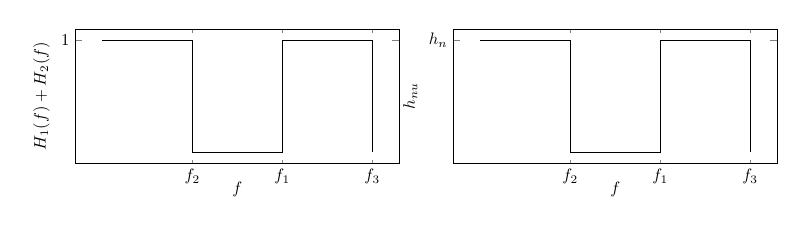
\begin{tikzpicture}[scale=.6]
		\begin{scope}
		\begin{axis}[xtick={1,2,3},xticklabels={$f_2$,$f_1$,$f_3$},ytick={1,2,3,4},xlabel=$f$,ylabel=$H_1(f)+H_2(f)$,yscale=.5]
		\addplot[black] coordinates {(0,1)(1,1)(1,0)(2,0)(2,1)(3,1)(3,0)};
		\end{axis}
		\end{scope}
		\begin{scope}
		\begin{axis}[xshift=8cm,xtick={1,2,3},xticklabels={$f_2$,$f_1$,$f_3$},ytick={1},yticklabel={$h_n$},xlabel=$f$,ylabel=$h_{nu}$,yscale=.5]
		\addplot[black] coordinates {(0,1)(1,1)(1,0)(2,0)(2,1)(3,1)(3,0)};
		\end{axis}
		\end{scope}
		\end{tikzpicture}}
	
	\subfloat[$f_2 < f_1$]{
		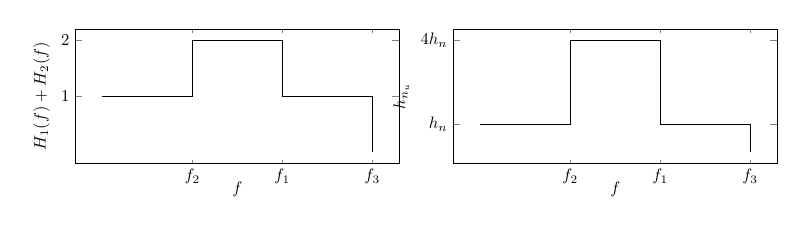
\begin{tikzpicture}[scale=.6]
		\begin{scope}
		\begin{axis}[xtick={1,2,3},xticklabels={$f_2$,$f_1$,$f_3$},ytick={1,2},xlabel=$f$,ylabel=$H_1(f)+H_2(f)$,yscale=.5]
		\addplot[black] coordinates {(0,1)(1,1)(1,2)(2,2)(2,1)(3,1)(3,0)};
		\end{axis}
		\end{scope}
		\begin{scope}
		\begin{axis}[xshift=8cm,xtick={1,2,3},xticklabels={$f_2$,$f_1$,$f_3$},ytick={1,4},ytick={1,4},yticklabels={$h_n$,$4h_n$},xlabel=$f$,ylabel=$h_{n_u}$,yscale=.5]
		\addplot[black] coordinates {(0,1)(1,1)(1,4)(2,4)(2,1)(3,1)(3,0)};
		\end{axis}
		\end{scope}
		\end{tikzpicture}}
\end{figure}
\end{esempio}

\begin{esempio}
Si abbia un apparato TV con fattore di rumore $F_\text{TV}=\SI{10}{\decibel}$ (ovvero una attenuazione $\alpha=10 \quad\alpha_\text{dB}=10\Log\alpha=10$). Un cavo collega l'antenna alla TV ha una attenuazione $\alpha_\text{dB}=\SI{3}{\decibel}$.

Si calcoli il fattore di rumore del sistema ricevente. Come si può abbassarlo a $\SI{6}{\decibel}$?
\begin{figure}[!ht]
	\centering
	\begin{circuitikz}[scale=.8]
		\draw (0,0) node[antenna,label=left:Antenna]{} to[short,label=$F_1$] (4,0) node[draw,block,label=above:$F_\text{TV}$]{$TV$};
		\draw [decorate,decoration={brace,amplitude=10pt,mirror},yshift=-12pt] (0,0)-- node [black,pos=.5,yshift=-20pt] {ampl. $\frac{1}{\alpha}$} (3,0);
	\end{circuitikz}
\end{figure}

L'attenuatore passivo che attenua di $\alpha_\text{dB}=\SI{3}{\decibel}$ dimezza la potenza $\alpha=2$ (amplifica di $1/2$).

Il fattore di rumore del sistema in catena di amplificazione:
\[F_S=F_1+F_2=\alpha+\frac{F_\text{TV}-1}{1/\alpha}=2+\frac{10-1}{1/2}=20\]
Espresso in decibel $10\Log 20=10\Log 2\cdot 10=10\Log 2+10\Log 10=(3+10)\si{\decibel}=\SI{13}{\decibel}$.

Per ridurre il fattore di rumore da $\SI{13}{\decibel}$ a $\SI{6}{\decibel}$ è necessario inserire un amplificatore a monte del cavo che collega l'antenna al TV, dove il segnale arriva debole e prima dell'attenuazione del cavo.
\begin{figure}[!ht]
	\centering
	\begin{circuitikz}[scale=.8]
		\draw (0,0) node[antenna,label=left:Antenna]{} to[short] (1,0) node[draw,block,label=above:$F_A$]{$A, T_a$} to[short,label=$F_2$] (5,0) node[draw,block,label=above:$F_\text{TV}$]{$TV$};
		\draw [decorate,decoration={brace,amplitude=10pt,mirror},yshift=-12pt] (2,0)-- node [black,pos=.5,yshift=-20pt] {ampl. $\frac{1}{\alpha}$} (4,0);
	\end{circuitikz}
\end{figure}
Si ottiene una catena di amplificazione a tre stadi con fattore di rumore:
\[F_S=F_A+F_2+F_\text{TV}=F_A+\frac{\alpha-1}{A}+\frac{F_\text{TV}-1}{A/\alpha}\leq 4 \quad(F_S\leq\SI{6}{\decibel})\]
\[F_S=F_A+\frac{2-1}{A}+\frac{10-1}{A/2}=F_A+\frac{1}{A}+\frac{18}{A}=F_A+\frac{19}{A}\leq 4\]
Si deve scegliere l'amplificatore con il guadagno $A$ minore che soddisfi la disequazione e eviti la saturazione e conseguente distorsione del segnale.
\end{esempio}
